% Metódy inžinierskej práce

\documentclass[10pt,slovak,a4paper]{article}

\usepackage[slovak]{babel}
%\usepackage[T1]{fontenc}
\usepackage[IL2]{fontenc} % lepšia sadzba písmena Ľ než v T1
\usepackage[utf8]{inputenc}
\usepackage{graphicx}
\usepackage{url} % príkaz \url na formátovanie URL
\usepackage{hyperref} % odkazy v texte budú aktívne (pri niektorých triedach dokumentov spôsobuje posun textu)
\usepackage{pdfpages}
\usepackage{cite}
\usepackage{dirtytalk}
\usepackage{indentfirst}
%\usepackage{times}

\graphicspath{ {./graphics/} }

\pagestyle{headings}

\title{Nový spôsob vzdelávania pomocou fenoménov\thanks{Semestrálny projekt v predmete Metódy inžinierskej práce, ak. rok 2020/21, vedenie: Mgr. Martin Sabo, PhD.}} % meno a priezvisko vyučujúceho na cvičeniach

\author{Rastislav Brna\\[2pt]
	{\small Slovenská technická univerzita v Bratislave}\\
	{\small Fakulta informatiky a informačných technológií}\\
	{\small \texttt{xbrna@stuba.sk}}
	}

\date{\small 30. september 2020} % upravte



\begin{document}

\maketitle

\begin{abstract}
	Vzdelávanie pomocou fenoménov je vzdelávanie v ktorom neexistujú 
	tradičné predmety ale vzdeláva sa na základe väčších tém ktoré sa rozoberajú zo všetkých strán.
	Jednu tému vieme rozobrať z fizikálneho, geografického, matematického, dejepisného alebo iného 
	hladiska. Tento štýl vzdelávania by mal zlepšit pochopenie učiva, keďze ludzký mozog vie spájať 
	si súvislosti medzi vecami omnoho lepšie ako si pamätať fakty naspamäť. V niektorých krajinách ktoré
	patria medzi lídrov vo vzdelávaní sa takýto systém už pomaly začína používať v praxi. Štúdia z turecka,
	potvrdila zlepšenie priemeru študentov o viac ako 10\%. Taktiež tento typ vzdelávania pomohol študentom 
	si dlhšie zachovať znalosťi ktoré nadobudly.\cite{jcer553507} 
\end{abstract}

\section{Úvod}

Svet a technológie idú dopredu ale sposob vzdelávanie je zastaralý a stovky rokov rovnaký. Znalosti potrebné k
životu sa menia a preto sa potrebuje prispôsobiť aj vzdelávanie. Aktuálny vzdelávací systém vo väčšine krajín 
rozdeluje vzdelávanie na určité smery(predmety), núti študentov sa učit vaľa veci z pamäti, vyvíja zbytočný tlak
a nezmyselne stresuje študentov už od útleho veku. Vzdelávanie na základe
fenoménov (Phenomenon-Based Learning) je metódou vzdelávania ktorá by mala zvýšit efektivitu vzdelávania
a dodať študentom lepšiu zručnosť, kreativitu, kritické myslenie, a schopnosť koloaborovať. Závisí na študovaní
fenoménu reálneho sveta z rôznych smerov pomocou čoho prepája hranice medzi školskými predmetami ako ich poznáme.
Mení vysvetlovanie novej látky z vysvetlenia učiva, vhoršom prípade len napísania poznámok z látky na tabulu na úvádzanie
študentov do témy cez zauhjímavé príbehy alebo hry a nabádanie ich k otázkam vďaka ktorým si znalosť témy osvoja a hlbšie zapametajú.
Aktívne núti študentov kolaborovať medzi sebov a zúčastnovať sa na spoločných aktivitách za účelom riešenia
problémov a odpovedania na otázky. 

\section{Výsledky štúdii}

\subsection{Turecko}

Štúdia z turecka \cite{jcer553507} skúmala vzdelávanie na základe fenoménov pre vyučovanie Informačných a komunikačných technológií
kôli chýbajúcemu praktickému využitiu tohoto predmetu. Na troch rôznych základných školách vybrali zo siedmej, ôsmej a deviatej
triedy spolu 121 študentov. V ôsmej triede bolo iba okolo 8 študentov, takže jej výsledok môže byť ovplyvnený lepším pomerom studentov
k učitelom. Študentov rozdelili na dve skupiny, jedna sa vzdelávala tradičným spôsobom a v druhej sa testovalo vzdelávanie na základe
fenoménov. Na konci štúdia dostali študenti k vypracovaniu test.

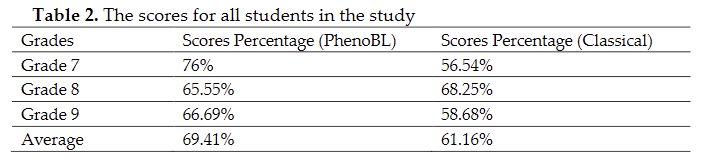
\includegraphics [width=0.9\textwidth] {table.png}

Ako ukazuje tabulka, úspešnosť je v priemero o 8\% vyššia pri vzdelávaní na základe fenoménov ako pri tradičnom vzdelávaní, avšak v 
ôsmej triede je úspešnosť vyššia pri tradičnom vzdelávaní. Toto môže byť zapríčinené či už veľmi malou vzorkov študentov alebo je
tradičné vzdelávanie pri velmi dobrom pomere žiakov k učitelom lepšie, pretože sa tam nájde viac priestoru pre zapájanie sa študentov,
čo tradičné vzdelávanie velmi vylepší. Takýto scenár je ajtak veľmi nereálny keďže možnosť vyrtvárať takto extrémne malé triedy môže byť iba
na súkromných školách.

Neskôr po teste študenti vypĺnali dotazník kde mali uviesť či by vedeli použiť znalosti a zručnosťi ktoré nadobudly počas štúdia. Približne 53\%
študentov odpovedalo že by ich dokázali použiť. To indikuje že použitie vzdelávania na základe fenoménov pomáha študentom použiť nadobudnuté 
znalosti a zručnosti omnoho dlhšie.

\subsection{Indonézia}

%TODO
\cite{Santhalia_2020}

\section{Skúsenosti z praxe}

%TODO
\cite{pblf}

\section{Záver}

Výsledký o vzdelávaniana základe fenoménov nachádzajú zlepšenie vo výsledkoch študentov. Fínsko po implementácii
tohoto vzdelávacieho systému priamo do školstva v celej krajine sa stále drží medzi top krajinami na svete a zaznamenalo 
nárast úspešnosti študentov. Systém sa javý ako veľkým zlepšením oproti predchádzajúcemu avšak úpravu budú potrebujú aj
štandardizované testy ktoré su priamo viazané na naspameť fakty na ktoré nieje kladený z dobrých dôvodov dôraz.

\bibliography{literature}
\bibliographystyle{apalike}

\end{document}
